\setchapterpreamble[o]{%
  \dictum[Benjamin Disraeli]{\textit{``There are three kinds of lies: lies, damn
    lies, and statistics''}}}

\chapter{Results}
\label{cha:results}

\begin{figure}[h]
  \begin{center}
    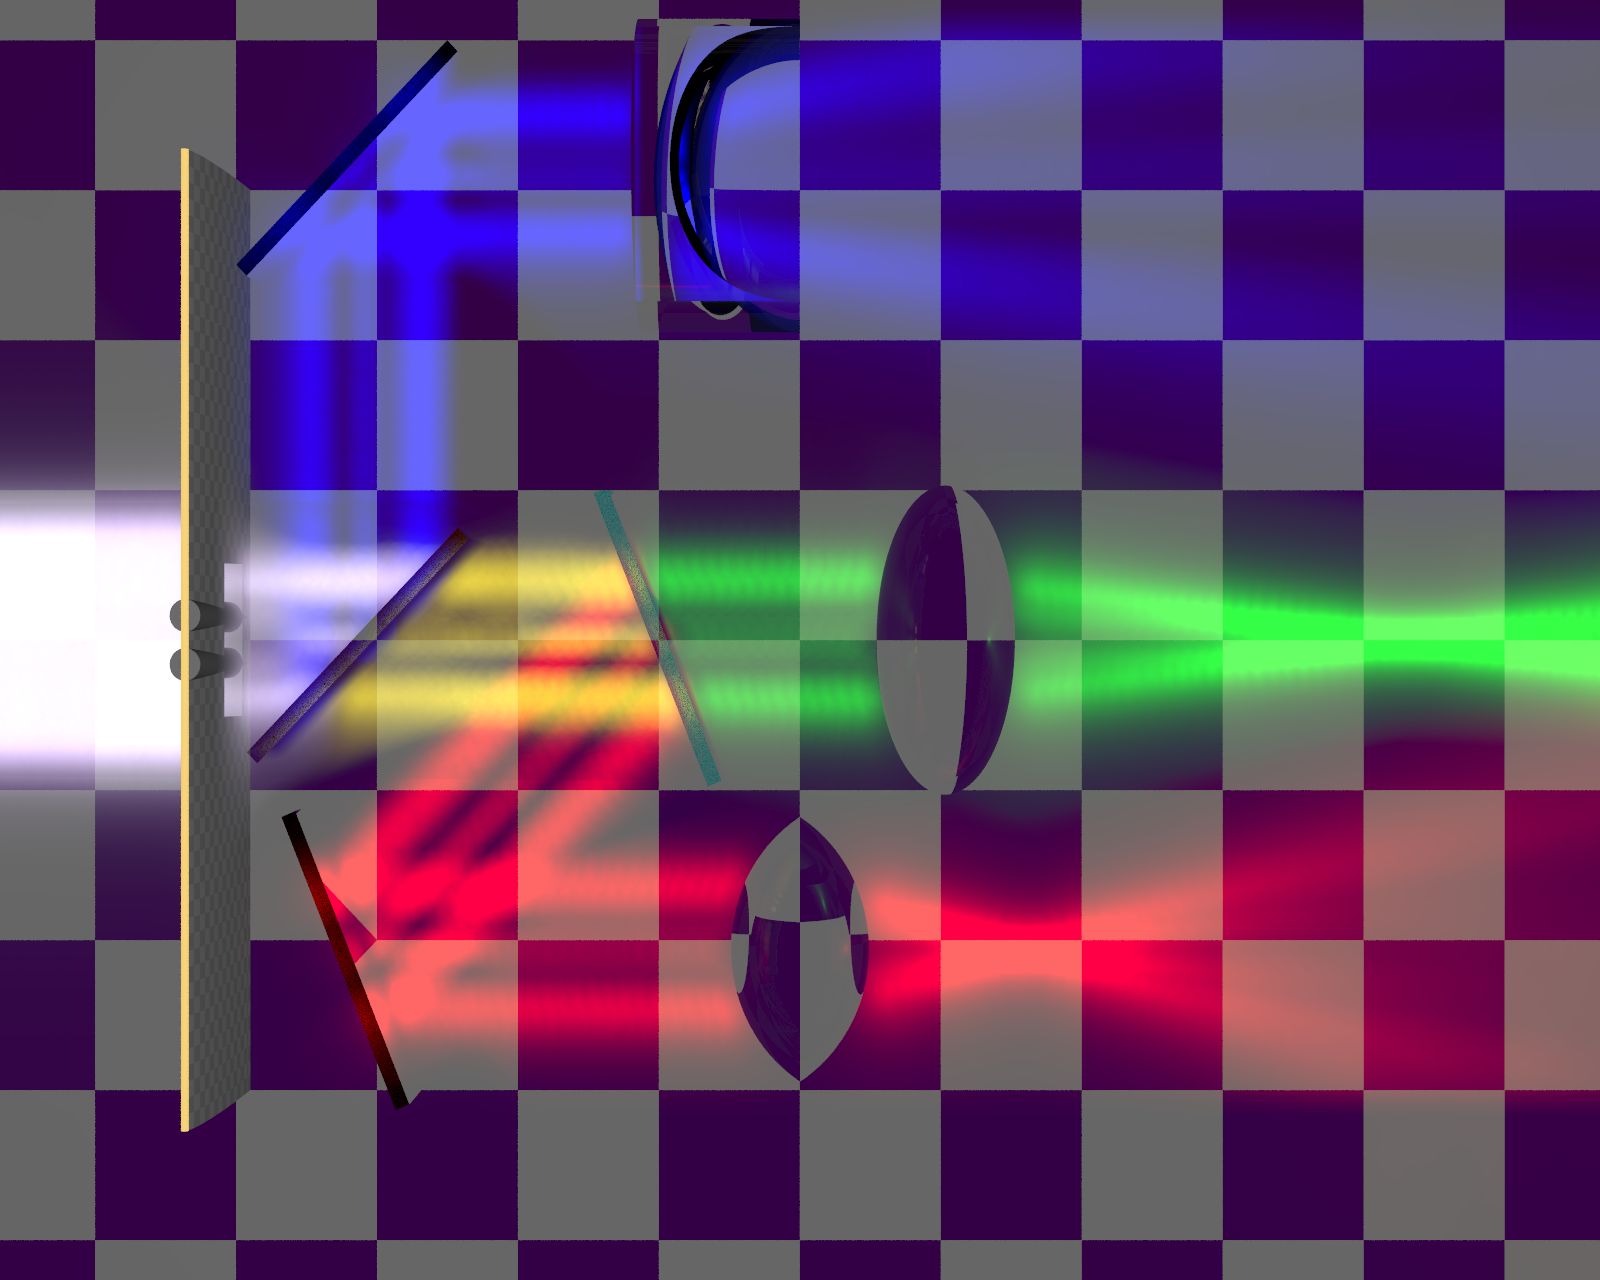
\includegraphics[height=5cm]{povray/optics}
  \end{center}
  \caption[An advanced POV-Ray picture]{TODO: fill me in}
  \label{fig:pov-optics}
\end{figure}

\section{Hello World!}
\label{sec:hello-world}

\section{Complex Computation}
\label{sec:complex-example}


\section{The Benefits of Data Caching}
\label{sec:data-caching}

 \begin{figure}
   \subfigure[POV-Ray example without cache]{
     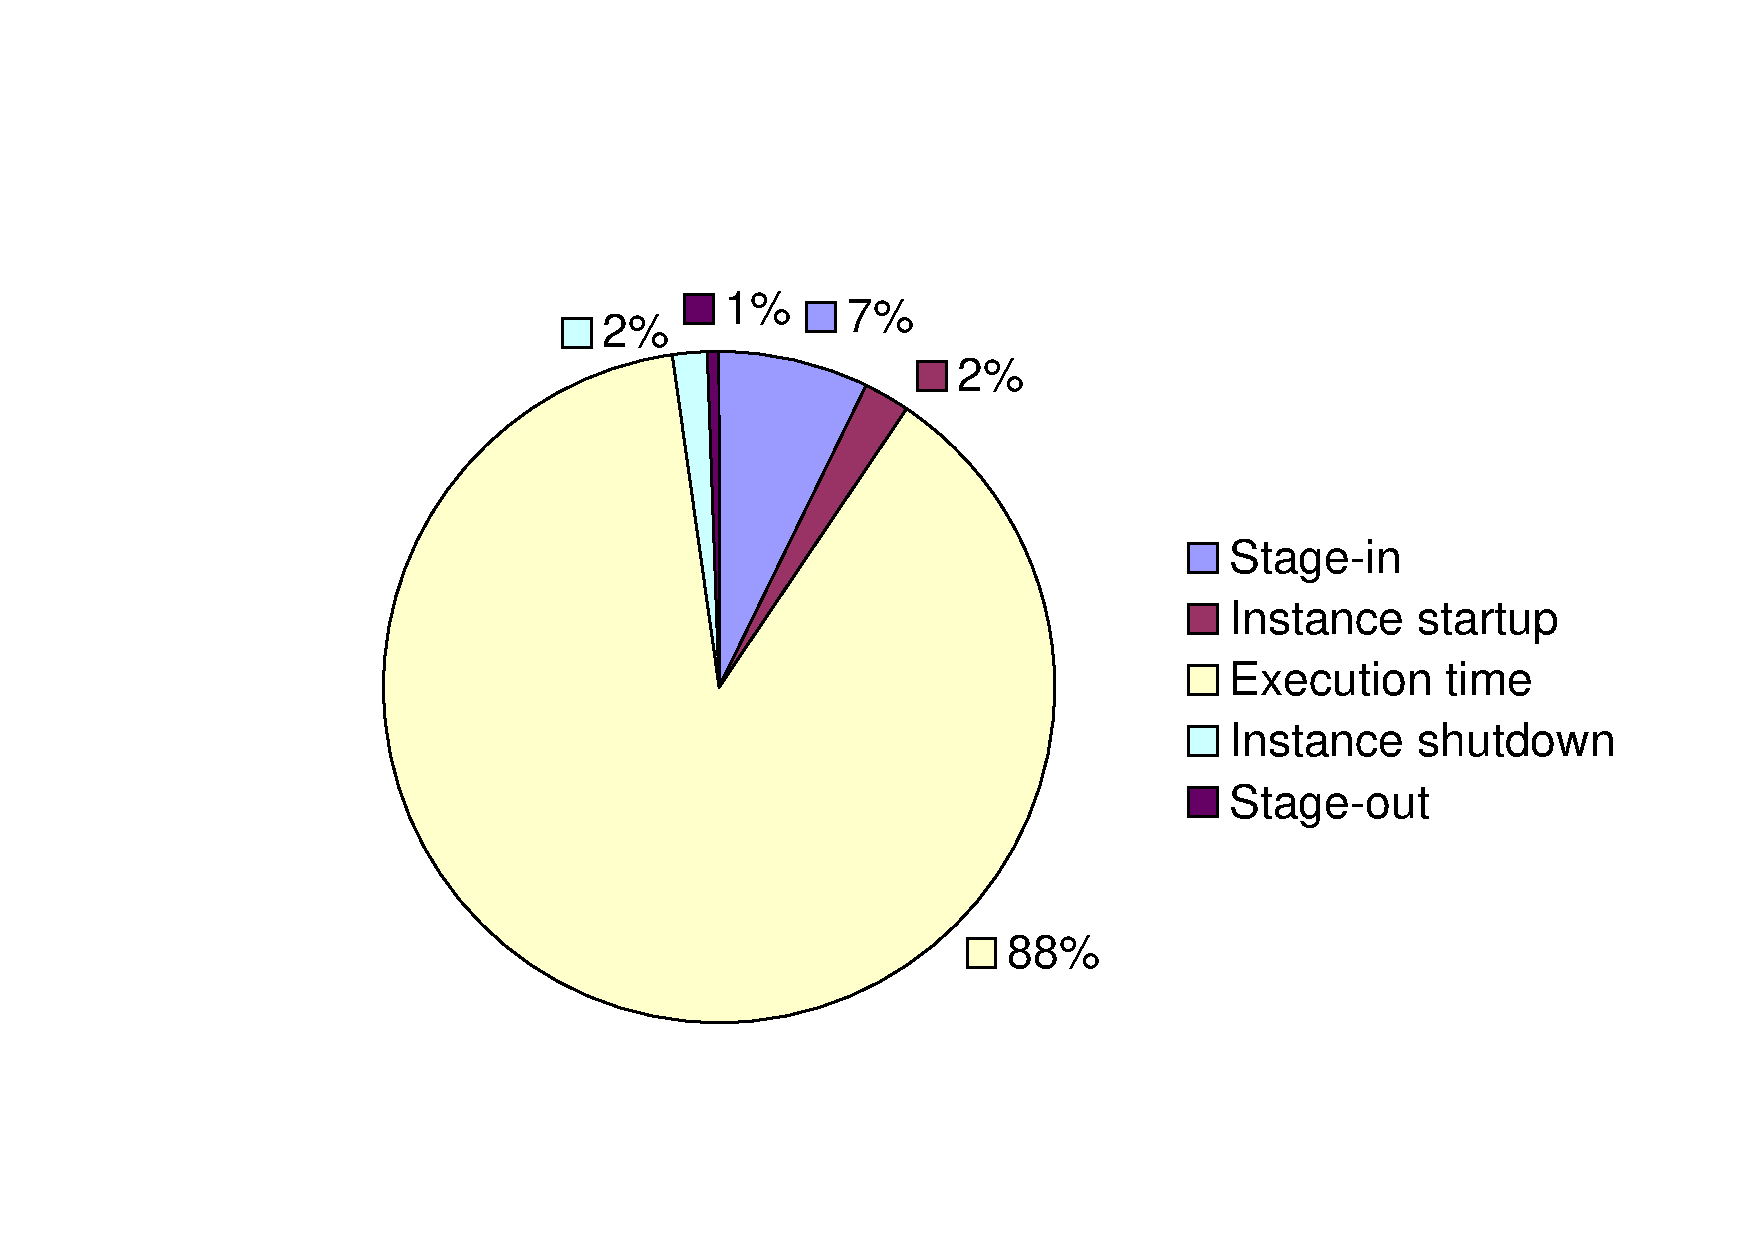
\includegraphics[width=.45\textwidth]{results/povray-nocache}
   }
   \subfigure[POV-Ray example with cached image]{
     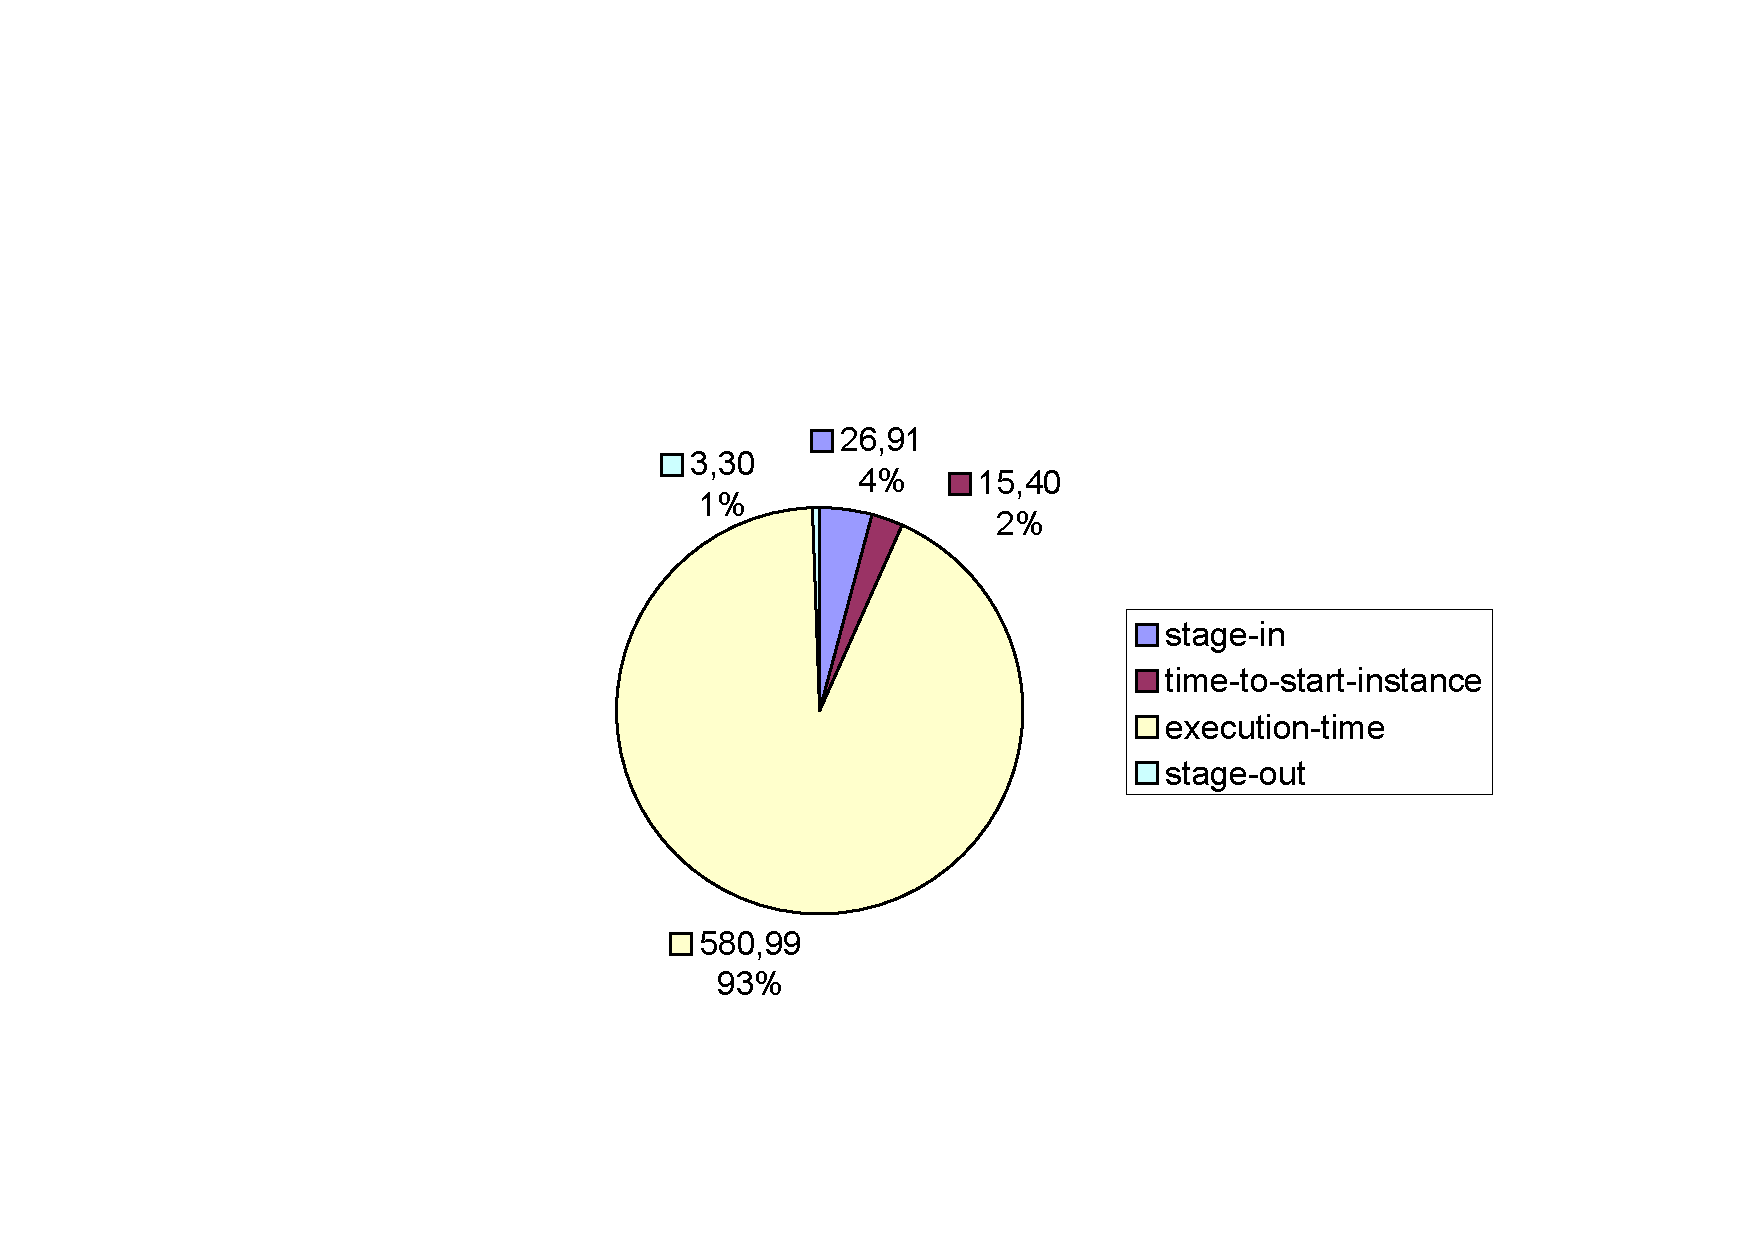
\includegraphics[width=.45\textwidth]{results/povray-cache}
   }
   \label{fig:pov-cache-comparison}
   \caption{Comparison of POV-Ray job with and without cache usage.}
\end{figure}

\begin{figure}[ht]
  \centering
  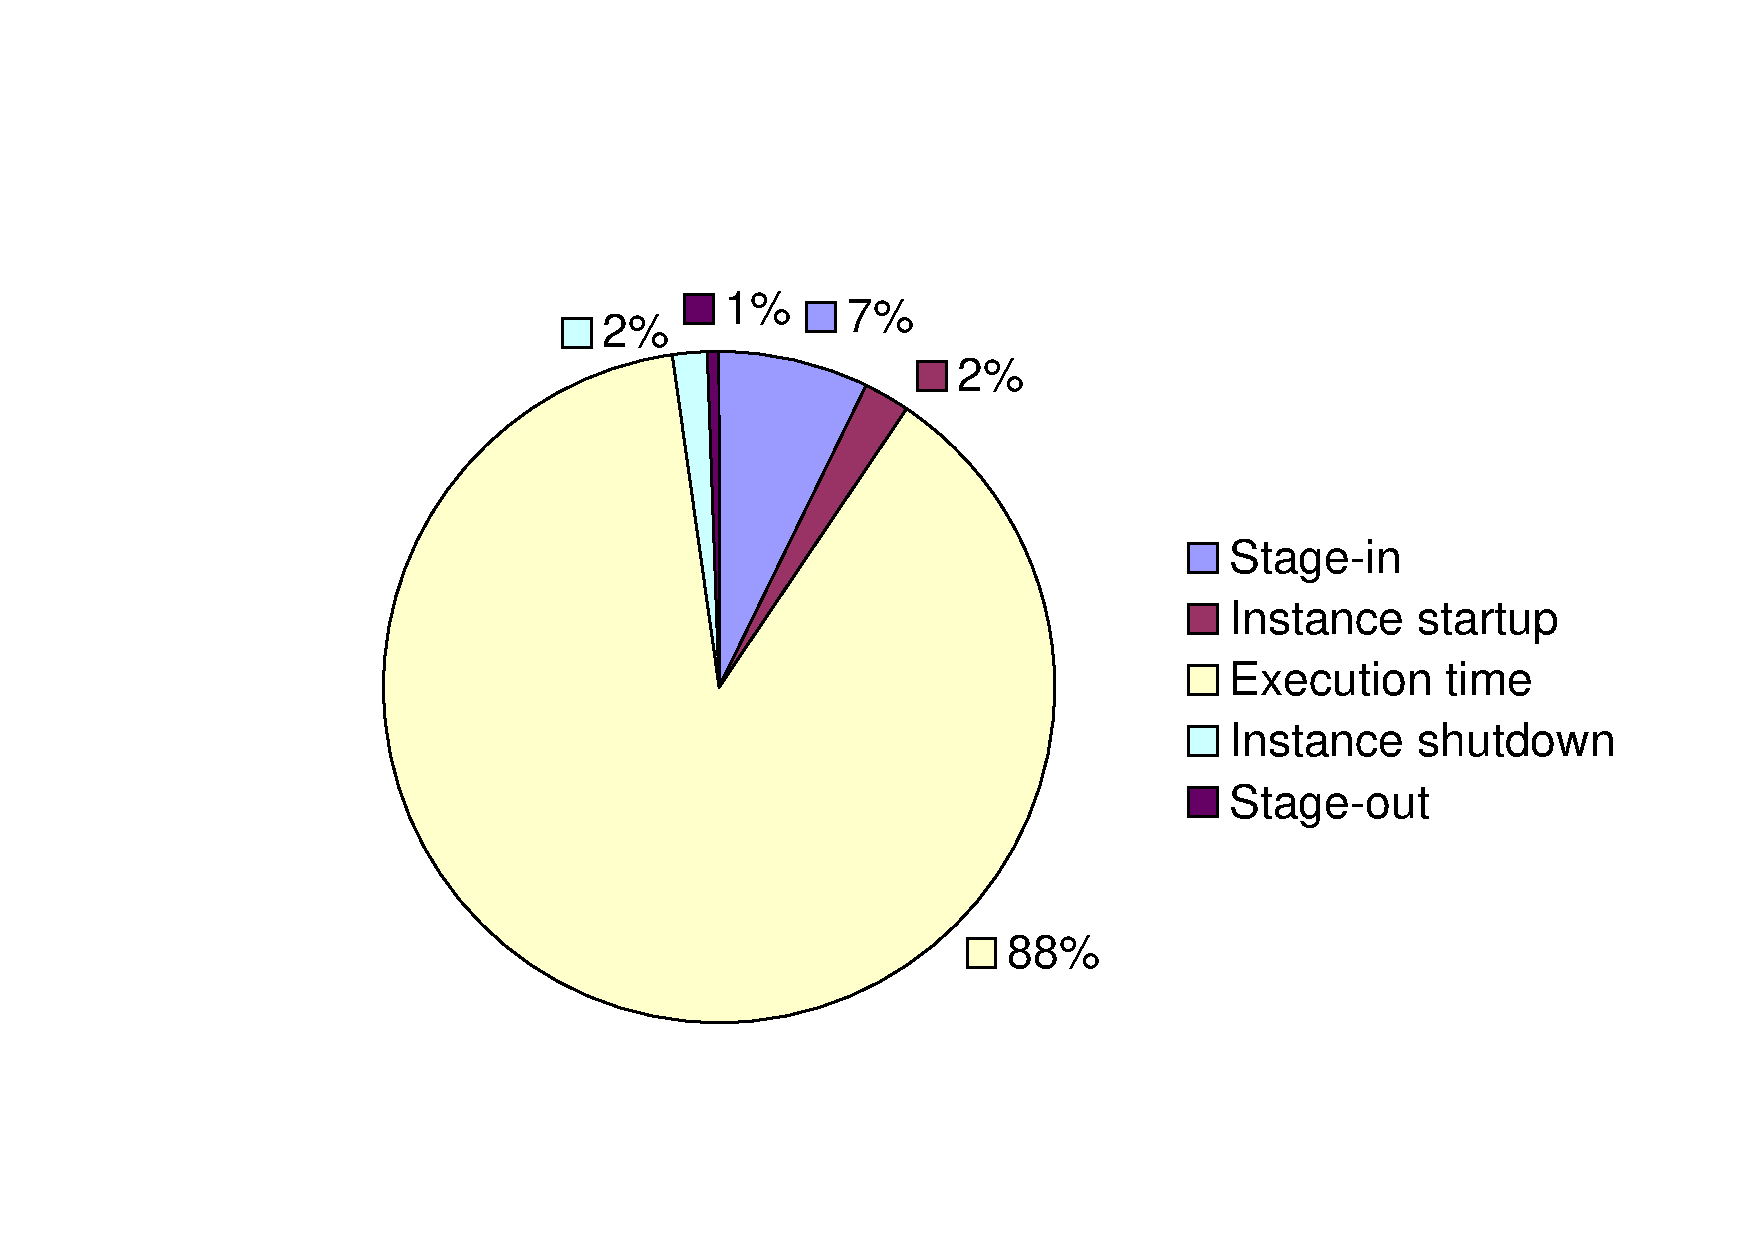
\includegraphics[width=.45\textwidth]{results/povray-nocache}
  \caption{POV-Ray example without cache}
  \label{fig:povray-nocache}
\end{figure}

\begin{figure}[ht]
  \centering
  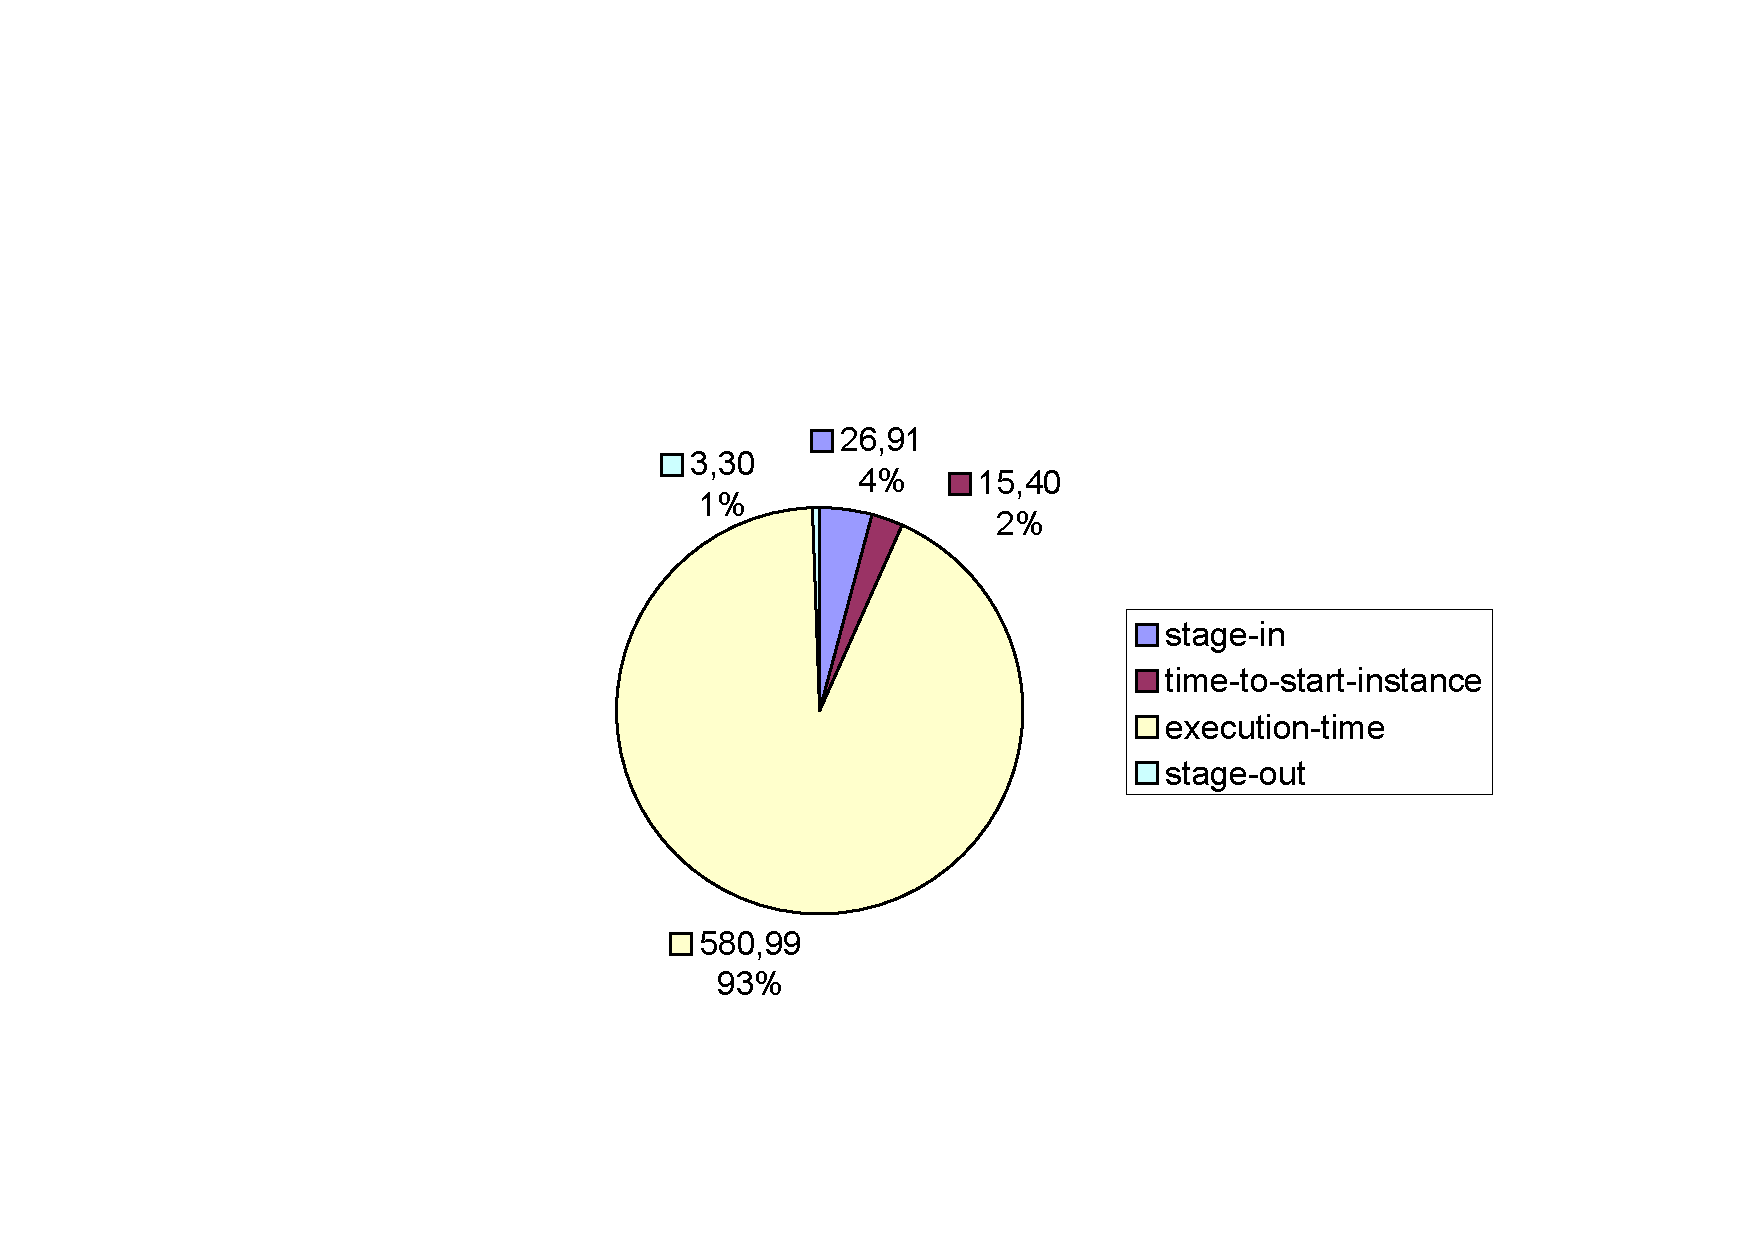
\includegraphics[width=.45\textwidth]{results/povray-cache}
  \caption{POV-Ray example with cache}
  \label{fig:povray-cache}
\end{figure}

\section{On-demand Server Deployment}
\label{sec:on-demand-server-deployment}

\subsection{SSH login}


%%% Local Variables: 
%%% mode: latex
%%% TeX-master: "main"
%%% End: 
